\documentclass{article}

\usepackage{times}
\usepackage{geometry}
\geometry{a4paper,left=0.6cm,right=0.7cm,top=1cm,bottom=1cm,columnsep=0.8cm}

\usepackage{fontawesome}
\usepackage[hidelinks]{hyperref}
\usepackage{multicol,paracol,tikz,hyphsubst,moresize,hyphenat,adjustbox,tabularx,xcolor,enumitem}
\newcolumntype{Y}{>{\RaggedRight\arraybackslash}X}
\setlist[itemize]{itemsep=1pt,leftmargin=*,topsep=-10pt}

\definecolor{maincolor}{HTML}{ffffff}
\definecolor{seccolor}{HTML}{0b1f3b}
\definecolor{gray}{HTML}{8c94a9}
\definecolor{sidetext}{HTML}{59cee5}
\definecolor{Green}{HTML}{2caf00}
\definecolor{lightgray}{HTML}{D3D3D3}

% --- bande latérale bleue
\usepackage{eso-pic}
\AddToShipoutPictureBG{%
  \begin{tikzpicture}[remember picture,overlay]
    \fill[seccolor] (0.7\paperwidth,0) rectangle (\paperwidth,\paperheight);
    \fill[maincolor] (0,0) rectangle (0.7\paperwidth,\paperheight);
  \end{tikzpicture}%
}

\setlength{\parindent}{0pt}
\newcommand{\cvsection}[1]{%
  \par\bigskip                % espace avant le titre
  {\bfseries\Large #1}\par
  \noindent\rule{\linewidth}{0.8pt}\par
  \medskip                    % espace après la ligne
}

\newcommand*{\ClipSep}{0.4cm}

% ------------------------------------------------------------------
\begin{document}\pagestyle{empty}
\columnratio{0.7}\begin{paracol}{2}

% --------- colonne gauche -----------------------------------------
\begin{minipage}{0.7\linewidth}
{\LARGE\textbf{Judikaël Mourouvin}}

\bigskip
{\large\textbf{Technicien informatique \& marketing digital}}
\end{minipage}\hfill
\begin{minipage}{0.18\linewidth}
\begin{tikzpicture}
\node[inner sep=0pt]{ 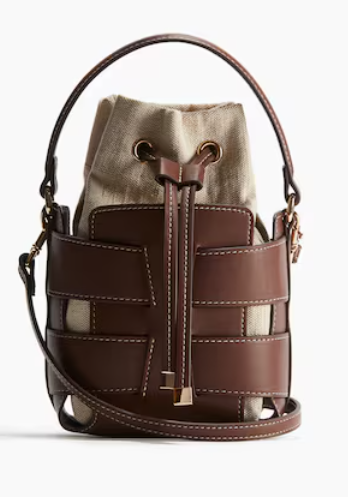
\includegraphics[width=\linewidth]{dad398677585422ea50b8320cf3f864a.png} };
\draw[white,rounded corners=\ClipSep,line width=\ClipSep]
      (current bounding box.north west) --
      (current bounding box.north east) --
      (current bounding box.south east) --
      (current bounding box.south west) -- cycle;
\end{tikzpicture}
\end{minipage}

\cvsection{Profil}
Passionné par l’informatique et le marketing digital, je maîtrise la configuration de postes, la maintenance et le diagnostic d’incidents. Mon alternance à la DSI de la Mairie du Gosier m’a permis de gérer des projets numériques et de former les utilisateurs. Rigoureux, autonome et orienté solution, je souhaite désormais mettre mes compétences au service de nouveaux défis à temps plein.

\cvsection{EXPÉRIENCE}

\colorbox{maincolor}{%
  \begin{minipage}{\linewidth}
    \textbf{Alternant en marketing digital} \\ Mairie du Gosier, DSI \\ 2023-2024
    \begin{itemize}
      \item Participé à la gestion de projets numériques pour la DSI, assurant leur avancement \item Analysé les besoins des utilisateurs et déployé des solutions adaptées \item Assuré le support technique et formé les agents tout en contribuant à la stratégie digitale
    \end{itemize}
  \end{minipage}}

\vspace{3mm}


\colorbox{maincolor}{%
  \begin{minipage}{\linewidth}
    \textbf{Animateur de la zone informatique} \\ Pôle Emploi, Gosier \\ 2022-2023
    \begin{itemize}
      \item Fourni une assistance technique quotidienne aux demandeurs d’emploi \item Configuré et entretenu les postes de travail pour garantir leur disponibilité \item Diagnostiqué et résolu les incidents pour optimiser la qualité du service
    \end{itemize}
  \end{minipage}}

\vspace{3mm}


\colorbox{maincolor}{%
  \begin{minipage}{\linewidth}
    \textbf{Stagiaire informaticien} \\ Numerika, Baie-Mahault \\ 2020-2021
    \begin{itemize}
      \item Configuré et maintenu les équipements informatiques de l’entreprise \item Assuré le support utilisateurs pour garantir la continuité des opérations \item Contribué à la résolution rapide des pannes matérielles et logicielles
    \end{itemize}
  \end{minipage}}

\cvsection{FORMATION}

    \begin{tabularx}{\linewidth}{@{}c X@{}}
    \textcolor{sidetext}{\faGraduationCap} &
    \textbf{Bachelor Marketing Digital} \\
    & CFA IUTS \\
    & \begin{itemize}[leftmargin=*]
  \item Étude des stratégies de communication digitale et des réseaux sociaux \item Apprentissage du référencement, de l’analytique web et de la gestion de projet marketing
\end{itemize} \\
    & \textit{2023-2024}
    \end{tabularx}
    

\vspace{3mm}


    \begin{tabularx}{\linewidth}{@{}c X@{}}
    \textcolor{sidetext}{\faGraduationCap} &
    \textbf{BTS Système Numérique option Informatique et Réseaux} \\
    & Lycée de Chevalier Saint Georges, Abymes \\
    & \begin{itemize}[leftmargin=*]
  \item Formation aux architectures réseau, systèmes et sécurité \item Pratique de la maintenance, du diagnostic et de l’assistance technique
\end{itemize} \\
    & \textit{2019-2021}
    \end{tabularx}
    

% --------- colonne droite (bleue) ---------------------------------
\switchcolumn\color{white}\hspace*{0.4cm}\begin{minipage}{0.88\linewidth}

\cvsection{CONTACT}
\begin{tabular}{@{}c l}
  \faPhone & \href{tel:+5900690911448}{+5900690911448} \\[2pt]
  \faEnvelope & \href{mailto:jkmou971@gmail.com}{jkmou971@gmail.com} \\[2pt]
  \faMapMarker & Route de Cocoyer\,97190 Gosier \\[2pt]
  \faLinkedin & \href{}{}
\end{tabular}

\cvsection{COMPÉTENCES}

\begin{itemize}[leftmargin=*]
\item Administration
\item Réseaux
\item Support
\item Maintenance
\item Marketing
\item Diagnostic
\item Configuration\end{itemize}
\par\bigskip 

\cvsection{LANGUES}
\begin{itemize}[leftmargin=*]
\item English - \textcolor{gray}{}
\item Español - \textcolor{gray}{}\end{itemize}
\par\bigskip 
\cvsection{INTÉRÊTS}
\begin{itemize}[leftmargin=*]
\item Lecture \& veille technologique
\item Randonnée / sports outdoor
\item Voyages \& découverte culturelle
\end{itemize}

\end{minipage}
\end{paracol}
\end{document}
